\documentclass[12pt]{beamer}
\usetheme[navbar=false, bkgimage=false, shadow=true]{Fermi}

\usepackage{graphicx}

\usepackage{amsmath}

\title{A New Maximum Likelihood Method for Defining the pulsar off-peak}
%\subtitle{\ldots}

\author{Joshua Lande\\[1em]
With much help from Damien + Matthew}
\institute{SLAC/Stanford}
\email{joshualande@gmail.com}
\date{August 25, 2011}

\begin{document}

\fermititle

\begin{frame}{Motivation}
  \begin{itemize}
    \item Most People like to study where the pulsar is
    \item But many reason to want to know where (in phase) the pulsar is not
      \begin{itemize}
        \item Studying nearby sources which may be confused $\rightarrow$ $\gamma$-Cgygni SNR
        \item Off-peak emission (or lack therefo) is interesting for pulsar modeling  $\rightarrow$ CTA1
        \item Looking for DC emission from the pulsar's wind $\rightarrow$ PWNCAT2
      \end{itemize}
  \end{itemize}
\end{frame}

\begin{frame}{What has been done before}

  lala

  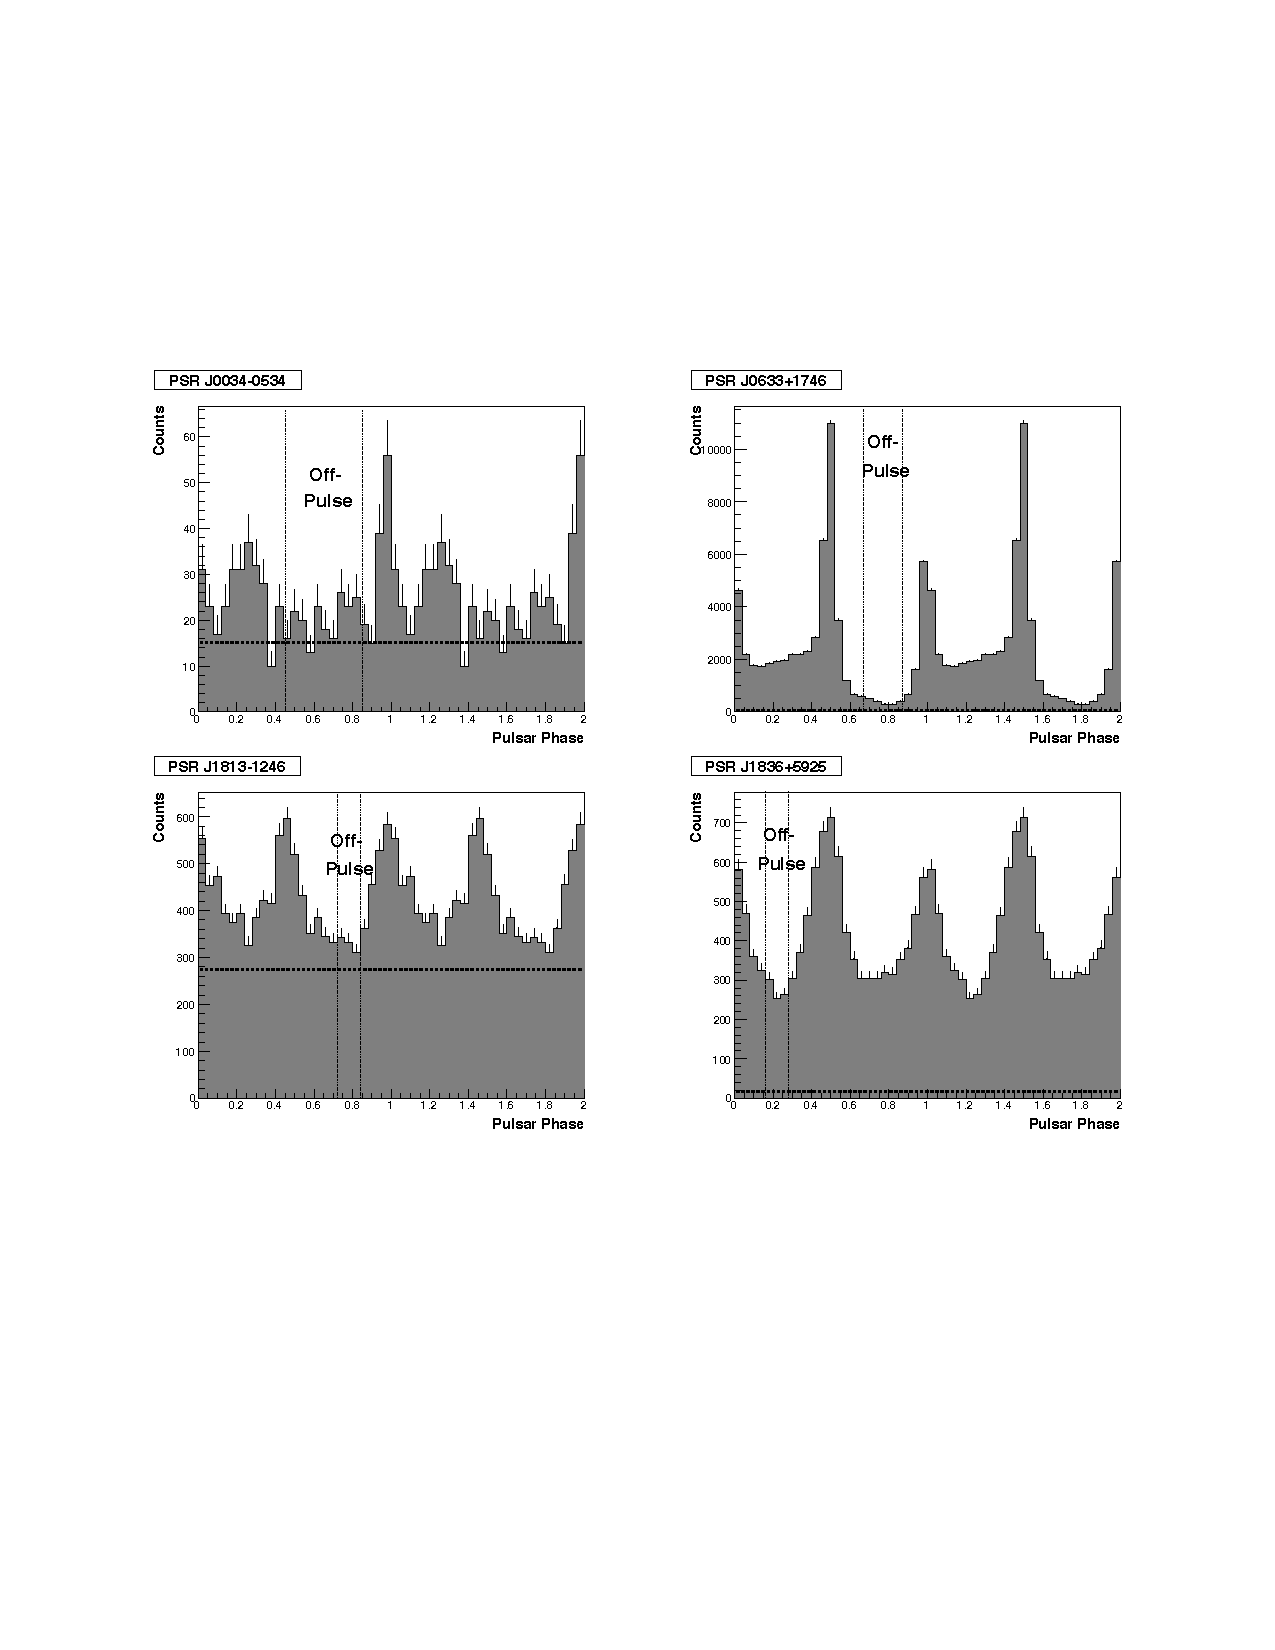
\includegraphics[width=0.75\textwidth]{plots/off_pulse_pwncat1.pdf}

  PWNCat1 $\rightarrow$ Selected by eye using pulsar phaseogram.
\end{frame}

\begin{frame}{Another Method: CTA1-Paper II}
  lala

  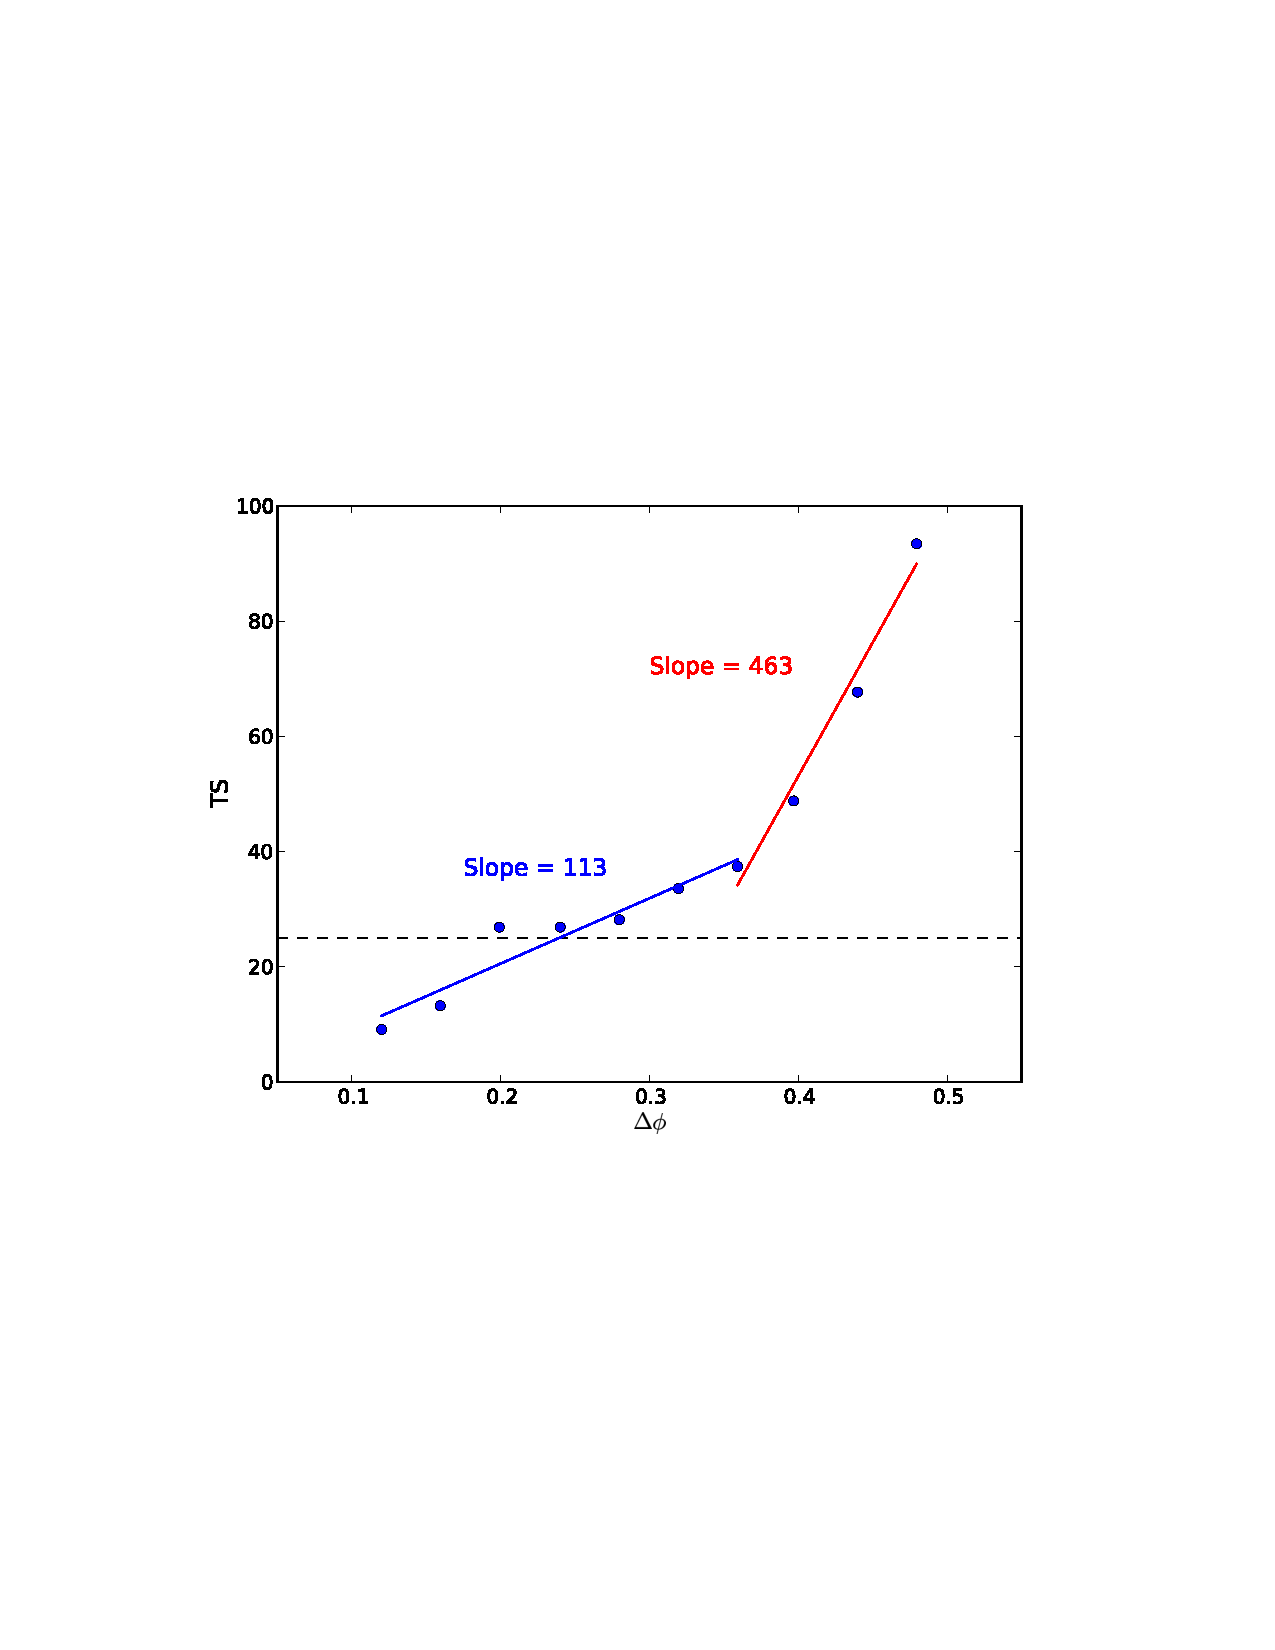
\includegraphics[width=0.75\textwidth]{plots/cta1.pdf}

  2nd CTA1 Paper$\rightarrow$ Look for break in TS vs $\Delta \phi$

\end{frame}

\begin{frame}{Maximum likelihood pulsar fitting}
  \begin{itemize}
    \item New idea for how to define the off pulse, proposed by Matthew
Background
   \item \texttt{uw.pulsar} for maximum likelihood fitting of pulsar light curves
   \item Has to be done anyway for 2nd pulsar catalog (Damien + Matthew)
     do define the peak separations
   \item Idea, can we use the best fit light curve to define the off peak?
  \end{itemize}
\end{frame}

\begin{frame}{\texttt{uw.pulsar}, under the hood}
  \begin{itemize}
   \item Define the likelihood: $\mathcal{L} = \sum_\text{photons}\text{PDF}(\text{phase})$
   \item Here, $\text{PDF}=\text{PDF}(\text{model parameters})$, so you have to pick a pulsar light curve model!
   \item As usual, maximize the log of the Likelihood
  \end{itemize}

  Example:\footnote{From \url{https://confluence.slac.stanford.edu/x/2AIyAw}}
  \begin{columns}
    \column{0.5\textwidth}
    \center{2 Gaussian}

    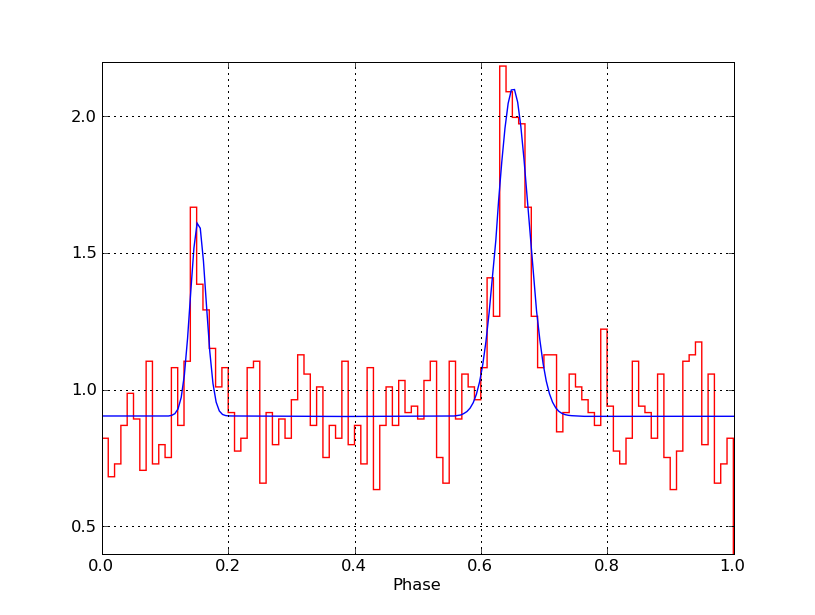
\includegraphics[width=1\textwidth]{plots/template_example_gauss.png}

    \column{0.5\textwidth}
    \center{2 Lorenzians}
    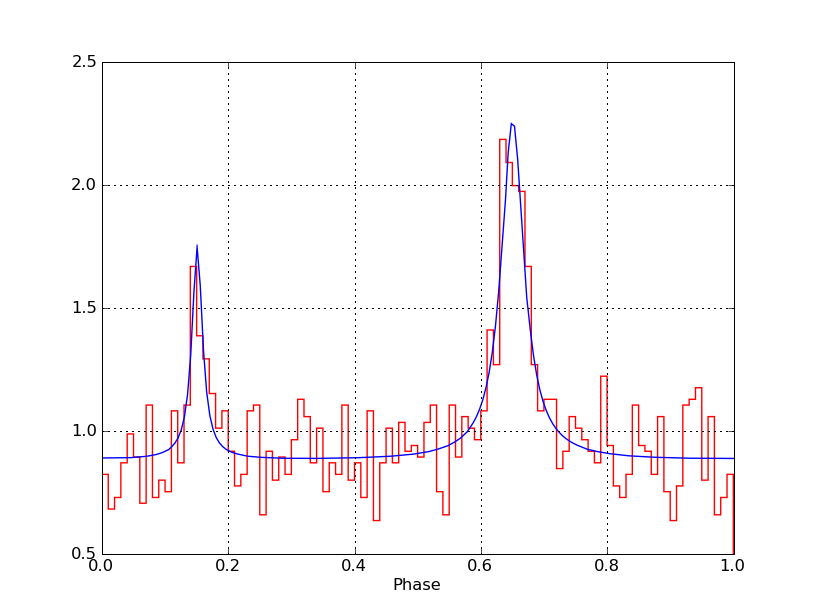
\includegraphics[width=1\textwidth]{plots/template_example_lorentzian.png}
  \end{columns}
\end{frame}

\begin{frame}{A more complicated Exmaple}
  \begin{itemize}
    \item Vela:
  \end{itemize}

\end{frame}

\end{document}
